
% Szkielet dla pracy inżynierskiej pisanej w języku polskim.

\documentclass[polish,masters,a4paper,twoside]{ppfcmthesis}


\usepackage[utf8]{inputenc}
\usepackage[OT4]{fontenc}
\usepackage{algorithm}
\usepackage{algorithmic}
\usepackage{listings}

\usepackage{rotating}
\usepackage{pdfpages}

% Authors of the thesis here. Separate them with \and
\author{Wiktor Latanowicz \album{66271}}
\authortitle{}                                        % Do not change.
\title{Framework do tworzenia aplikacji internetowych uruchamianych w środowisku przeglądarki}                   % Note how we protect the final title phrase from breaking
\ppsupervisor{dr inż. Rafał Różycki} % Your supervisor comes here.
\ppyear{2013}                                         % Year of final submission (not graduation!)

\lstset{basicstyle=\small, breakindent=40pt, breaklines}
\lstdefinelanguage[Objective]{C}[GNU99]{C}
  {morekeywords={@catch,@class,@encode,@end,@finally,@implementation,%
      @interface,@private,@protected,@protocol,@public,@selector,%
      @synchronized,@throw,@try,BOOL,Class,IMP,NO,Nil,SEL,YES,_cmd,%
      bycopy,byref,id,in,inout,nil,oneway,out,self,super,%
      % The next two lines are Objective-C 2 keywords.
      @dynamic,@package,@property,@synthesize,readwrite,readonly,%
      assign,retain,copy,nonatomic%
      },%
   moredirectives={import}%
  }%
\lstdefinelanguage[GNU99]{C}[99]{C}
  {morekeywords={asm,__asm__,__extension__,typeof,__typeof__}%
  }%
\lstdefinelanguage[99]{C}%
  {morekeywords={_Bool,_Complex,_Imaginary,auto,break,case,char,%
      const,continue,default,do,double,else,enum,extern,float,for,%
      goto,if,inline,int,long,register,restrict,return,short,signed,%
      sizeof,static,struct,switch,typedef,union,unsigned,void,volatile,%
      while},%
   sensitive,%
   morecomment=[s]{/*}{*/},%
   morecomment=[l]//,%
   morestring=[b]",%
   morestring=[b]',%
   moredelim=*[directive]\#,%
   moredirectives={define,elif,else,endif,error,if,ifdef,ifndef,line,%
      include,pragma,undef,warning}%
  }[keywords,comments,strings,directives]%
  
  
\begin{document}

% Front matter starts here
\frontmatter\pagestyle{empty}%
\maketitle\cleardoublepage%

% Blank info page for "karta dyplomowa"
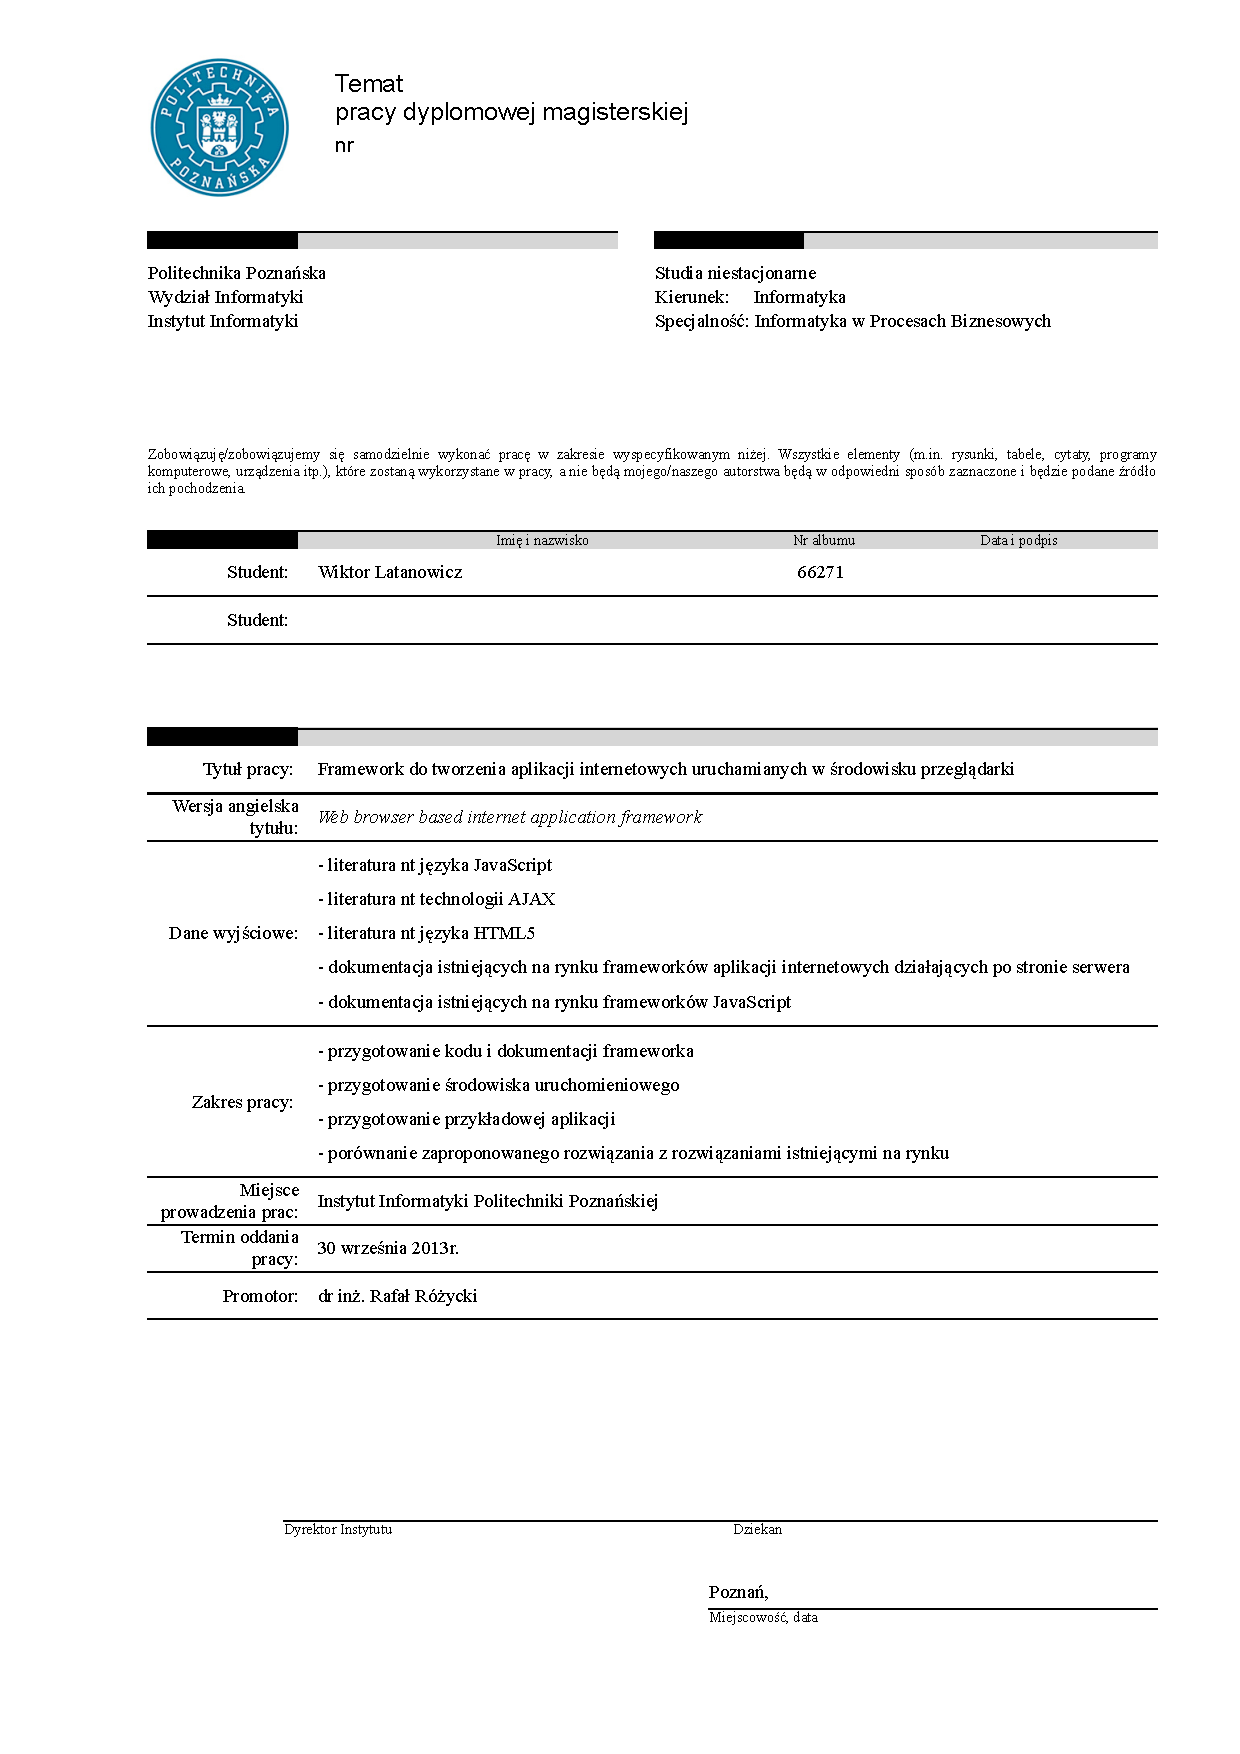
\includepdf{figures/karta}
\cleardoublepage%

% Table of contents.
\pagenumbering{Roman}\pagestyle{ppfcmthesis}%
\tableofcontents* \cleardoublepage%

% Main content of your thesis starts here.
\mainmatter%

\chapter{Wstęp}


\chapter{Motywacja}

Od dłuższego czasu zaobserwować można trend, w którym aplikacje kierowane dla biznesu
migrują w kierunku rozwiązań opartych na WWW. Do niedawna ubogie możliwośći techniczne
przeglądarek oraz częste problemy z implementacją standardów przez autorów przeglądarek
w znaczący sposób utrudniały tworzenie interaktywnych aplikacji bazujących na technologiach
internetowych. Rozwiązaniem problemów ułomności przeglądarek internetowych było
przeniesienie kodu aplikacji odpowiedzialnego za interfejs użytkownika na serwer aplikacyjny.
Przy takim podejściu przeglądarka była zwolniona z wykonywania, nierzadko rozbudowanego,
kodu odpowiedzialnego za warstwę prezentacji. Dodatkowym atutem rozwiązania była możliwość
dostarczenia wersji interfejsu dostosowanej do konkretnej przeglądarki. Użytkownik korzystający
z przeglądarki wspierającej najnowsze standardy mógł korzystać z lepszej, bardziej
interaktywnej wersji interfejsu. Z drugiej strony możliwe było wykrycie, że oprogramowanie,
z którego korzysta użytkownik nie spełnia wymagań i przesłanie mu uboższej, lecz działającej
w jego środowisku, wersji interfejsu.

Pomimo licznych zalet rozwiązanie, w którym cały interfejs użytkownika jest w całości
przygotowywany na serwerze ma bardzo istotną z punktu widzenia użytkownika wadę ---
brak interaktywności. Każda czynność wykonana przez użytkownika w interfejsie aplikacji
wymagała wysłania przesłania zapytania na serwer, przetworzenia tego zapytania i odesłania
do przeglądarki zaktualizowanego interfejsu użytkownika. W całości.

Wraz z rozwojem i ustandaryzowaniem w przeglądarkach internetowych wsparcia dla języków
skryptowych takich jak JavaScript autorzy aplikacji internetowych wzbogacali je o elementy
interaktywne. Wykorzystanie koncepcji AJAX, zastosowanej po raz pierwszy pod koniec lat
90-tych XX wieku, pozwoliło także na wymianę danych pomiędzy interfejsem aplikacji a
serwerem bez konieczności przeładowywania całej strony.

Naturalnym kierunkiem rozwoju aplikacji internetowych było całkowite przeniesienie generowania
interfejsu aplikacji do przeglądarki internetowej. Wielu autorów bibliotek ułatwiających
pisanie interaktywnych aplikacji internetowych zauważyło ten fakt. Powstało wiele licznych
rozwiązań ułatwiających modyfikowanie, czy wręcz tworzenie od zera, interfejsu aplikacji
w środowisku przeglądarki. Rozwiązania takie jak funkcje ułatwiające przeszukiwanie i
modyfikacje drzewa DOM, ułatwienia obsługi zdarzeń, czy wykorzystanie szablonów w znaczny
sposób ułatwiają tworzenie aplikacji, których interfejs użytkownika w znacznej części
powstaje w komputerze użytkownika.

Zdaniem autora niniejszej pracy, dostępnym obecnie na rynku bibliotekom JavaScript, ułatwiającym
tworzenie interaktywnych aplikacji, daleko pod kątem prostoty użycia do ewoluujących od lat
rozwiązań serwerowych takich jak Microsoft WebForms czy Ruby on Rails. Ideą, którą kierowano
się w niniejszej pracy było stworzenie lekkiego frameworka, działającego w środowisku przeglądarki,
który stawiałby programistom podobnie niskie wymagania co nowoczesne rozwiązania serwerowe.
Dodatkowym wymogiem było, w miarę możliwości, uniezależnienie od bibliotek zewnętrznych i
unikanie konfliktów z takimi bibliotekami.
\chapter{Projekt i implementacja systemu}

\chapter{Testowanie}


\chapter{Zakończenie}


\section{Podsumowanie}


\cleardoublepage\appendix%

\chapter{Diagram klas całego systemu}


\nocite{*}

% Bibliography (books, articles) starts here.
\bibliographystyle{plalpha}{\raggedright\sloppy\small\bibliography{bibliography}}

% Colophon is a place where you should let others know about copyrights etc.
\ppcolophon

\end{document}
